% Ensure included PDFs (banners) with newer versions embed without warnings
\pdfminorversion=7
\documentclass[aspectratio=169]{beamer}

\makeatletter
% Make LaTeX find theme .sty files in Template
\def\input@path{{../Template/}}
\makeatother
\usepackage{graphicx}
% Make graphics (including banner PDFs) resolvable without TEXINPUTS
\graphicspath{{../Template/}{../Template/banners/}{../../Common_Images/}}

%================================================================%
% Theme and Package Setup
%================================================================%
\usetheme{ucl}
\setbeamercolor{banner}{bg=darkpurple}

% Navigation and Footer
\setbeamertemplate{navigation symbols}{\vspace{-2ex}}
\setbeamertemplate{footline}[author title date]
\setbeamertemplate{slide counter}[framenumber/totalframenumber]

\usepackage[utf8]{inputenc}
\usepackage[british]{babel} % British spelling
\usepackage{amsmath, amssymb, amsthm}
\usepackage{graphicx}
\usepackage{tikz}
\usetikzlibrary{calc, positioning, arrows.meta, shapes.geometric, trees, backgrounds, shapes.misc, graphs, quotes, shadows, fit, patterns} 
\usepackage{pgfplots}
\pgfplotsset{compat=1.17}
\usefonttheme{professionalfonts}
\usepackage{eulervm}
\usepackage{listings}
\usepackage{algorithm}
\usepackage{algpseudocode}
\usepackage{xcolor}
\usepackage{subcaption}

% Define custom colours
\makeatletter
\@ifundefined{color@stone}{%
    \definecolor{stone}{gray}{0.95}%
}{}
\makeatother
\definecolor{darkgreen}{rgb}{0.0, 0.5, 0.0}
\definecolor{uclblue}{cmyk}{1,0.24,0,0.64}
\definecolor{uclred}{cmyk}{0,1,0.62,0}
\definecolor{uclpurple}{cmyk}{0.32,0.42,0,0.55}
\definecolor{uclorange}{cmyk}{0,0.45,0.91,0}
\definecolor{liftblue}{RGB}{27,79,114}
\definecolor{liftorange}{RGB}{201,116,32}
\definecolor{liftgreen}{RGB}{50,122,87}
\definecolor{liftred}{RGB}{168,54,54}
\definecolor{liftgrey}{RGB}{245,246,248}

\setbeamercovered{transparent}

% Define theoremblock
\makeatletter
\newenvironment<>{theoremblock}[1]{%
    \begin{block}#2{#1}%
}{\end{block}}
\makeatother

% Section divider slides
\AtBeginSection[]{
  \begin{frame}
    \frametitle{\textbf{\Large\insertsectionhead}}
    \begin{center}
        \huge\textbf{\insertsectionhead}
    \end{center}
  \end{frame}
}

% Maths Macros
\newcommand{\U}{\mathcal{U}}
\newcommand{\V}{\mathcal{V}}
\newcommand{\Z}{\mathcal{Z}}
\newcommand{\R}{\mathbb{R}}
\newcommand{\E}{\mathbb{E}}
\newcommand{\ip}[2]{\langle #1, #2 \rangle}
\newcommand{\norm}[1]{\| #1 \|}
\DeclareMathOperator*{\argmin}{argmin}
\DeclareMathOperator{\prox}{prox}
\DeclareMathOperator{\dom}{dom}
\DeclareMathOperator{\supremum}{sup}
\DeclareMathOperator{\sign}{sign}

% Semantic highlighting for this lecture
\newcommand{\standard}[1]{{\color{liftblue}#1}}
\newcommand{\relaxation}[1]{{\color{liftorange}#1}}
\newcommand{\bregman}[1]{{\color{liftgreen}#1}}
\newcommand{\failure}[1]{{\color{liftred}#1}}

% Reusable TikZ styles
\tikzset{
    statebox/.style={draw=black!20, rounded corners=2mm, fill=liftgrey, minimum width=1.8cm, minimum height=0.8cm, align=center},
    standardarrow/.style={-{Latex[length=2.5mm]}, very thick, draw=liftblue},
    backarrow/.style={-{Latex[length=2.5mm]}, ultra thick, draw=liftred},
    relaxarrow/.style={-{Latex[length=2.5mm]}, very thick, draw=liftorange},
    bregmanarrow/.style={-{Latex[length=2.5mm]}, very thick, draw=liftgreen},
    note/.style={font=\scriptsize, align=center}
}

\title{Lifted Neural Network Training}
\subtitle{Part 1: Foundations of Lifted Training and the Bregman Framework}
\author[Martin Benning (University College London)]{Martin Benning}
\date[COMP0263]{COMP0263 -- Solving Inverse Problems with Data-Driven Models \\[1cm] 17th March 2026}
\institute[]{University College London}

\begin{document}

% --- Title Frame ---
\begin{frame}
  \titlepage
\end{frame}

% --- Outline ---
\begin{frame}{Lecture Overview}
    \tableofcontents
\end{frame}

% ==============================================================================
\section{The Limitations of Standard Deep Learning Training}
% ==============================================================================

\begin{frame}{Recap: Empirical Risk Minimisation}
    Deep neural networks are standardly trained using gradient-based \textbf{empirical risk minimisation}.
    
    \vspace{0.5em}
    For a feed-forward neural network $\mathcal{N}$ parameterised by $\mathbf{\Theta} = \{\Theta_l\}_{l=1}^L$, the objective reads
    
    \begin{theoremblock}{Standard Training Objective}
    $$ \min_{\mathbf{\Theta}} \, \frac{1}{s}\sum_{i=1}^s \ell(y^i, \mathcal{N}(x^i, \mathbf{\Theta})) $$
    \end{theoremblock}
    \vspace{-0.1cm}
    Where:
    \begin{itemize}
        \item $s$ denotes the number of training samples.
        \item $(x^i, y^i)$ are the input and target pairs.
        \item $\ell$ signifies the loss function.
    \end{itemize}
\end{frame}

\begin{frame}{Deeply Nested Dependencies}
    \begin{columns}[T,totalwidth=\textwidth]
        \column{0.55\textwidth}
        Such models evaluate intermediate representations through recursive compositions
        \[
            x_l = \sigma_l(f(x_{l-1}, \Theta_l))
        \]
        so the prediction is obtained only after passing through the full chain of layers.

        \vspace{0.75em}
        \begin{alertblock}{Why this is structurally hard}
            Computing an update for an early parameter such as $\Theta_1$ requires information to travel through \emph{all} later layers first.
        \end{alertblock}

        \column{0.45\textwidth}
        \centering
        
        % Added \tikzset to ensure the custom styles compile successfully.
        \tikzset{
            statebox/.style={draw, rectangle, rounded corners=2pt, minimum size=6mm, inner sep=3pt},
            standardarrow/.style={->, >=stealth, thick},
            backarrow/.style={->, >=stealth, thick, dashed, red},
            note/.style={font=\scriptsize}
        }
        
        \begin{tikzpicture}[x=1cm,y=1cm,scale=0.7,transform shape]
            % Nodes (Ellipsis is now its own node for better spacing and logic)
            \node[statebox] (x0)   at (0,0)   {$x_0$};
            \node[statebox] (x1)   at (2.1,0) {$x_1$};
            \node[statebox] (x2)   at (4.2,0) {$x_2$};
            \node           (dots) at (6.0,0) {$\cdots$};
            \node[statebox] (x3)   at (7.8,0) {$x_L$};
            
            % Forward passes
            \draw[standardarrow] (x0) -- node[above,note] {$\Theta_1,\sigma_1$} (x1);
            \draw[standardarrow] (x1) -- node[above,note] {$\Theta_2,\sigma_2$} (x2);
            \draw[standardarrow] (x2) -- (dots);
            \draw[standardarrow] (dots) -- node[above,note] {$\Theta_L,\sigma_L$} (x3);
            
            % Back-propagated error chain
            % FIX: 'bend left' is used here so the right-to-left arrow curves underneath the nodes
            \draw[backarrow] (x3.south) to[bend left=25] node[below,note,align=center,text width=3.5cm] {back-propagated error chain} (x0.south);
        \end{tikzpicture}
    \end{columns}
\end{frame}

\begin{frame}{Standard Training via Back-Propagation}
    \begin{columns}[T,totalwidth=\textwidth]
        \column{0.48\textwidth}
        \textbf{Standard pipeline}
        \begin{itemize}
            \item forward pass through all layers,
            \item loss evaluation,
            \item full backward sweep through the chain rule,
            \item parameter update only afterwards.
        \end{itemize}

        \begin{center}
        \begin{tikzpicture}[x=1cm,y=1cm,scale=0.92]
            \node[statebox] (f) at (0,1.4) {forward};
            \node[statebox] (l) at (2.3,1.4) {loss};
            \node[statebox] (b) at (4.6,1.4) {backward};
            \node[statebox] (u) at (6.9,1.4) {update};
            \draw[standardarrow] (f)--(l);
            \draw[standardarrow] (l)--(b);
            \draw[backarrow] (b)--(u);
        \end{tikzpicture}
        \end{center}

        \column{0.48\textwidth}
        \textbf{What we want instead}
        \begin{itemize}
            \item layer variables made explicit,
            \item local subproblems rather than one nested chain,
            \item updates that can be parallelised,
            \item no differentiation through non-smooth activations.
        \end{itemize}

        \begin{center}
        \begin{tikzpicture}[x=1cm,y=1cm,scale=0.92]
            \node[statebox] (u1) at (0,1.4) {$x_1$};
            \node[statebox] (u2) at (2.3,1.4) {$x_2$};
            \node[statebox] (u3) at (4.6,1.4) {$x_3$};
            \draw[relaxarrow] (u1) -- (u2);
            \draw[relaxarrow] (u2) -- (u3);
            \draw[bregmanarrow] (u1) -- +(0,-1) node[below,note] {local penalty};
            \draw[bregmanarrow] (u2) -- +(0,-1) node[below,note] {local penalty};
            \draw[bregmanarrow] (u3) -- +(0,-1) node[below,note] {local penalty};
        \end{tikzpicture}
        \end{center}
    \end{columns}
\end{frame}

\begin{frame}{Fundamental Limitations of Back-Propagation}
    \begin{itemize}
        \item \textbf{Sequential Locking Bottleneck:} Its strictly sequential nature propagates errors layer-by-layer backwards through the chain rule. We cannot update layer 1 until the error has propagated through layer $L, L-1, \dots, 2$. This prevents massive parallelisation.
        \vspace{1em}
        \item \textbf{Numerical Instability:} Back-propagation can suffer from vanishing or exploding gradients, where weight updates become infinitesimally small or numerically unstable, especially in earlier layers of deep networks.
    \end{itemize}
\end{frame}

\begin{frame}{The Challenge of Non-Smooth Activations}
    Furthermore, modern architectures heavily rely on non-smooth activation functions such as the Rectified Linear Unit (ReLU).
    
    \vspace{1em}
    \begin{alertblock}{Sub-gradient Substitutions}
        Standard back-propagation inevitably requires sub-gradient substitutions at non-differentiable points (e.g., $x=0$ for ReLU). This mathematically compromises robust convergence rates compared to principled proximal minimisation approaches.
    \end{alertblock}
    
    \vspace{1em}
    \textbf{Goal:} Can we reformulate network training to avoid sequential back-propagation \textit{and} handle non-smooth activations natively?
\end{frame}

% ==============================================================================
\section{Distributed Optimisation \& The Method of Auxiliary Coordinates}
% ==============================================================================

\begin{frame}{Breaking the Sequential Chain}
    To circumvent the sequential nature of gradients, we can reformulate the learning process by introducing \textbf{auxiliary variables} that decouple the network layers.
    
    \vspace{1em}
    Define $x_l^i$ as the post-activation state of the $l$-th layer for sample $i$. We constrain these variables to satisfy the forward pass exactly:
    
    \begin{theoremblock}{Constrained Lifted Formulation}
    \begin{align*}
        \min_{\mathbf{\Theta}, \mathbf{X}} \, &\frac{1}{s}\sum_{i=1}^s \ell(y^i, x_L^i) \\
        \text{s.t.} \quad &x_l^i = \sigma_l(f(x_{l-1}^i, \Theta_l)) \quad \text{for } l = 1, \ldots, L
    \end{align*}
    \end{theoremblock}
\end{frame}

\begin{frame}{Method of Auxiliary Coordinates (MAC)}
    Relaxing these hard architectural constraints yields optimisation strategies that decouple the individual layers.
    
    \vspace{1em}
    A prominent strategy is the \textbf{Method of Auxiliary Coordinates (MAC)} \cite{CarreiraPerpinan2014}. MAC replaces the equality constraints with quadratic penalty terms.
    
    \begin{theoremblock}{MAC Objective}
    $$ \min_{\mathbf{\Theta}, \mathbf{X}} \frac{1}{s} \sum_{i=1}^{s} \left[ \ell(y^i, f(x_{L - 1}^i, \Theta_L)) + \sum_{l=1}^{L-1} \lambda_l \|x^i_{l} - \sigma_l(f(x_{l - 1}^i, \Theta_l)) \|_2^2 \right] $$
    \end{theoremblock}
    with penalty parameters $\lambda_l > 0$.
\end{frame}

\begin{frame}{Distributing the Workload}
    \begin{columns}[T,totalwidth=\textwidth]
        \column{0.52\textwidth}
        \begin{itemize}
            \item The nested problem is replaced by shallow, loosely coupled subproblems.
            \item This makes \textbf{block-coordinate descent} natural.
            \item Parameter groups and sample blocks can now be updated in parallel.
        \end{itemize}

        \vspace{0.5em}
        \begin{alertblock}{Remaining flaw}
            MAC still places $\sigma_l$ inside a quadratic penalty, so gradient-driven minimisation continues to differentiate the activation.
        \end{alertblock}

        \column{0.44\textwidth}
        \centering
        \begin{tikzpicture}[x=1cm,y=1cm]
            \foreach \i in {0,1,2} {
                \node[statebox, minimum width=1.8cm, minimum height=0.9cm] (a\i) at (0, -1.4*\i) {layer \the\numexpr\i+1\relax};
                \node[statebox, minimum width=1.8cm, minimum height=0.9cm, fill=orange!12] (b\i) at (3.2, -1.4*\i) {sample block};
                \draw[relaxarrow] (a\i) -- (b\i);
            }
            \node[note, align=center] at (1.6,1.0) {parallel shallow updates};
        \end{tikzpicture}
    \end{columns}
\end{frame}

% ==============================================================================
\section{The Classical Lifted Approach vs. The Bregman Framework}
% ==============================================================================

\begin{frame}{The Classical Lifted Approach}
    A second line of work observes that the ReLU activation function $\sigma(z) = \max(z, 0)$ itself can be viewed as the solution to a constrained minimisation problem.
    
    \vspace{1em}
    The activated output can be written as an orthogonal projection onto the non-negative orthant $\mathbb{R}_{+}^{n}$:
    $$ x_{l} = \sigma_l (W_l^\top x_{l-1} + b_{l}) = \argmin_{x \geq 0} \|x - (W_l^\top x_{l-1} + b_{l})\|_2^2 $$
    
    \vspace{1em}
    This implies that $x_l$ is the vector closest to $W_l^\top x_{l-1} + b_{l}$ that lies in the non-negative orthant.
\end{frame}

\begin{frame}{The Classical Lifted Objective}
    In the classical lifted approach \cite{askari2018lifted}, the constrained formulation is approximated by embedding the non-negativity constraint directly into the search space:
    
    \begin{theoremblock}{Classical Lifted Network Training}
    $$ \min_{\mathbf{\Theta},\{x_l^{i} \in \mathbb{R}_{+}^{n}\}_{l=1}^{L-1}} \frac{1}{s} \sum_{i=1}^{s} \left[ \ell(y^i, f(x^{i}_{L-1},\Theta_{L})) + \sum_{l=1}^{L-1} \|x^i_{l} - f(x^{i}_{l-1},\Theta_{l})\|_2^2 \right] $$
    \end{theoremblock}
    
    \vspace{1em}
    \begin{itemize}
        \item The search space is "lifted" to include auxiliary variables $x_l^i$.
        \item Each sub-problem is convex in each individual variable when keeping all others fixed.
        \item Updates use simple orthogonal projections onto the non-negative orthant.
    \end{itemize}
\end{frame}

\begin{frame}{The Fatal Flaw of Classical Lifting}
    \begin{columns}[T,totalwidth=\textwidth]
        \column{0.48\textwidth}
        \textbf{What we intended}
        \[
            x_l = \sigma_l(W_l^\top x_{l-1}+b_l)
        \]
        \begin{center}
        \begin{tikzpicture}[x=1cm,y=1cm]
            \node[statebox] (a) at (0,0) {$W_l^\top x_{l-1}+b_l$};
            \node[statebox, fill=green!10] (b) at (3.6,0) {$\sigma_l(\cdot)$};
            \draw[standardarrow] (a)--(b);
        \end{tikzpicture}
        \end{center}

        \column{0.48\textwidth}
        \textbf{What optimality forces}
        \[
            (W_l^\top x_{l-1}+b_l-x_l)=0
            \Longrightarrow
            \failure{x_l=W_l^\top x_{l-1}+b_l}
        \]
        \begin{alertblock}{Degeneracy at optimum}
            The nonlinearity is no longer active: the lifted model collapses to an affine-linear map.
        \end{alertblock}
    \end{columns}
\end{frame}

\begin{frame}{Enter the Bregman Framework}
    To circumvent the differentiation of non-smooth activation functions whilst maintaining distributed optimisation benefits \textit{without} degenerating to linear networks, we transition the penalty framework towards tailored \textbf{Bregman distances}.
    
    \vspace{1em}
    This framework mandates that activation functions be \textbf{proximal maps} of proper, convex and lower semi-continuous functions $\Psi$:
    $$ \sigma_l(z) = \operatorname{prox}_{\Psi}(z) = \argmin_{u} \left\{ \frac{1}{2} \| u - z \|_2^2 + \Psi(u) \right\} $$
\end{frame}

\begin{frame}{The Lifted Bregman Loss}
    \begin{columns}[T,totalwidth=\textwidth]
        \column{0.58\textwidth}
        By Fermat's rule, the proximal relation implies
        \[
            z - \sigma_l(z) \in \partial \Psi(\sigma_l(z)).
        \]
        Using the Fenchel conjugate, we define the \textbf{Bregman loss} \cite{WangBenning2023}:
        \begin{theoremblock}{Bregman Loss Definition}
        $$ B_{\Psi}(x, z) := \frac{1}{2}\|x\|_2^2 + \Psi(x) + \left(\frac{1}{2}\|\cdot\|_2^2 + \Psi\right)^*(z) - \langle x, z \rangle $$
        \end{theoremblock}
        
        \column{0.38\textwidth}
        \begin{block}{Interpretation}
            This is a \bregman{Fenchel--Young gap}. It is zero exactly when the architectural consistency condition is satisfied.
        \end{block}
        \vspace{0.5em}
        \begin{center}
        \begin{tikzpicture}[x=1cm,y=1cm]
            \node[statebox] (z) at (0,0) {pre-activation $z$};
            \node[statebox] (x) at (0,-1.5) {activation $x$};
            \draw[bregmanarrow] (z) -- node[right,note] {$B_\Psi$ enforces} (x);
        \end{tikzpicture}
        \end{center}
    \end{columns}
\end{frame}

\begin{frame}{Properties of the Bregman Loss}
    \begin{columns}[T,onlytextwidth]
        \column{0.32\textwidth}
        \begin{block}{\standard{1. Non-negative}}
            \[
                B_{\Psi}(x,z)\geq 0
            \]
            Equality holds exactly when $x=\prox_{\Psi}(z)$.
        \end{block}

        \column{0.32\textwidth}
        \begin{block}{\relaxation{2. Bi-convex}}
            Convex in $x$ for fixed $z$ and convex in $z$ for fixed $x$.

            \vspace{0.5em}
            This gives convex block subproblems.
        \end{block}

        \column{0.32\textwidth}
        \begin{block}{\bregman{3. Structurally richer}}
            It penalises both:
            \smallskip
            \begin{itemize}
                \item distance to $\sigma(z)$,
                \item violation of proximal structure.
            \end{itemize}
        \end{block}
    \end{columns}
\end{frame}

\begin{frame}{The Magic Gradient: Derivative-Free Updates}
    A critical property is the gradient of $B_\Psi$ with respect to its second argument. Differentiating the Fenchel conjugate and invoking the Moreau decomposition gives

    \vspace{0.5em}
    \begin{center}
        \setlength{\fboxsep}{8pt}
        \colorbox{green!10}{\parbox{0.68\textwidth}{
            \centering
            \Large $\nabla_z B_{\Psi}(x, z) = \sigma(z) - x$
        }}
    \end{center}

    \begin{alertblock}{Main computational payoff}
        Parameter updates require only \bregman{evaluating} $\sigma_l$ and comparing it with $x$; there is \failure{no derivative of the activation} anywhere in the update.
    \end{alertblock}
\end{frame}

\begin{frame}{The Lifted Bregman Training Problem}
    Incorporating $B_{\Psi}$ into the MAC framework by replacing the quadratic penalties yields the \textbf{Lifted Bregman} training problem:
    
    \begin{theoremblock}{Lifted Bregman Objective}
    $$ \min_{\mathbf{\Theta}, \mathbf{X}}  \sum_{i=1}^{s} \left[\ell\left(y^i, x_{L}^{i}\right) + \sum_{l=1}^{L-1} \,  \lambda_l B_{\Psi_l}\left(x_{l}^{i}, f(x_{l - 1}^{i}, \Theta_l) \right)\right] $$
    \end{theoremblock}
    
    This acts as a layer-wise Fenchel-Young consistency loss between activation variables and transformed pre-activations.
\end{frame}

\begin{frame}{Bregman Losses for Common Activations: ReLU}
    For ReLU, choose $\Psi(u) = \chi_{[0,\infty)^n}(u)$ (the indicator of the non-negative orthant), so that $\sigma(z)_j = \max(z_j, 0)$.
    
    $$ B_{\Psi}(x, z) = \begin{cases} \dfrac{1}{2}\|x - \max(z, 0)\|_2^2 + {\color{uclred}\langle x,\, \max(-z, 0)\rangle} & x \in [0,\infty)^n , \\[4pt] \infty & \text{otherwise.} \end{cases} $$
    
    \vspace{0.5em}
    Compared to the flawed quadratic penalty, the additional term ${\color{uclred}\langle x, \max(-z, 0)\rangle} \geq 0$ penalises configurations where $z$ has negative components. \textbf{This perfectly prevents the affine degeneracy!}
\end{frame}

\begin{frame}{Bregman Losses for Common Activations}
    \textbf{Soft-thresholding} ($\Psi(u) = \alpha |u |_1$ with $\alpha > 0$):
    $$ B_{\Psi}(x, z) = \begin{cases} \dfrac{1}{2}z^2 - z(\alpha + x) & z > \alpha , \\[4pt] -xz & |z| \leq \alpha , \\[4pt] \dfrac{1}{2}z^2 + z(\alpha - x) & z < -\alpha . \end{cases} $$
    
    \vspace{1em}
    \textbf{Hyperbolic tangent} (chosen such that $\sigma(z) = \tanh(z)$):
    $$ B_{\Psi}(x, z) = \begin{cases} \dfrac{1}{2}\log\!\left(\dfrac{1 - x^2}{1 - \tanh^2(z)}\right) + x\bigl(\tanh^{-1}(x) - z\bigr) & |x| < 1 , \\[4pt] \infty & \text{otherwise.} \end{cases} $$
\end{frame}

\begin{frame}{Proximal Activations at a Glance}
    \centering
    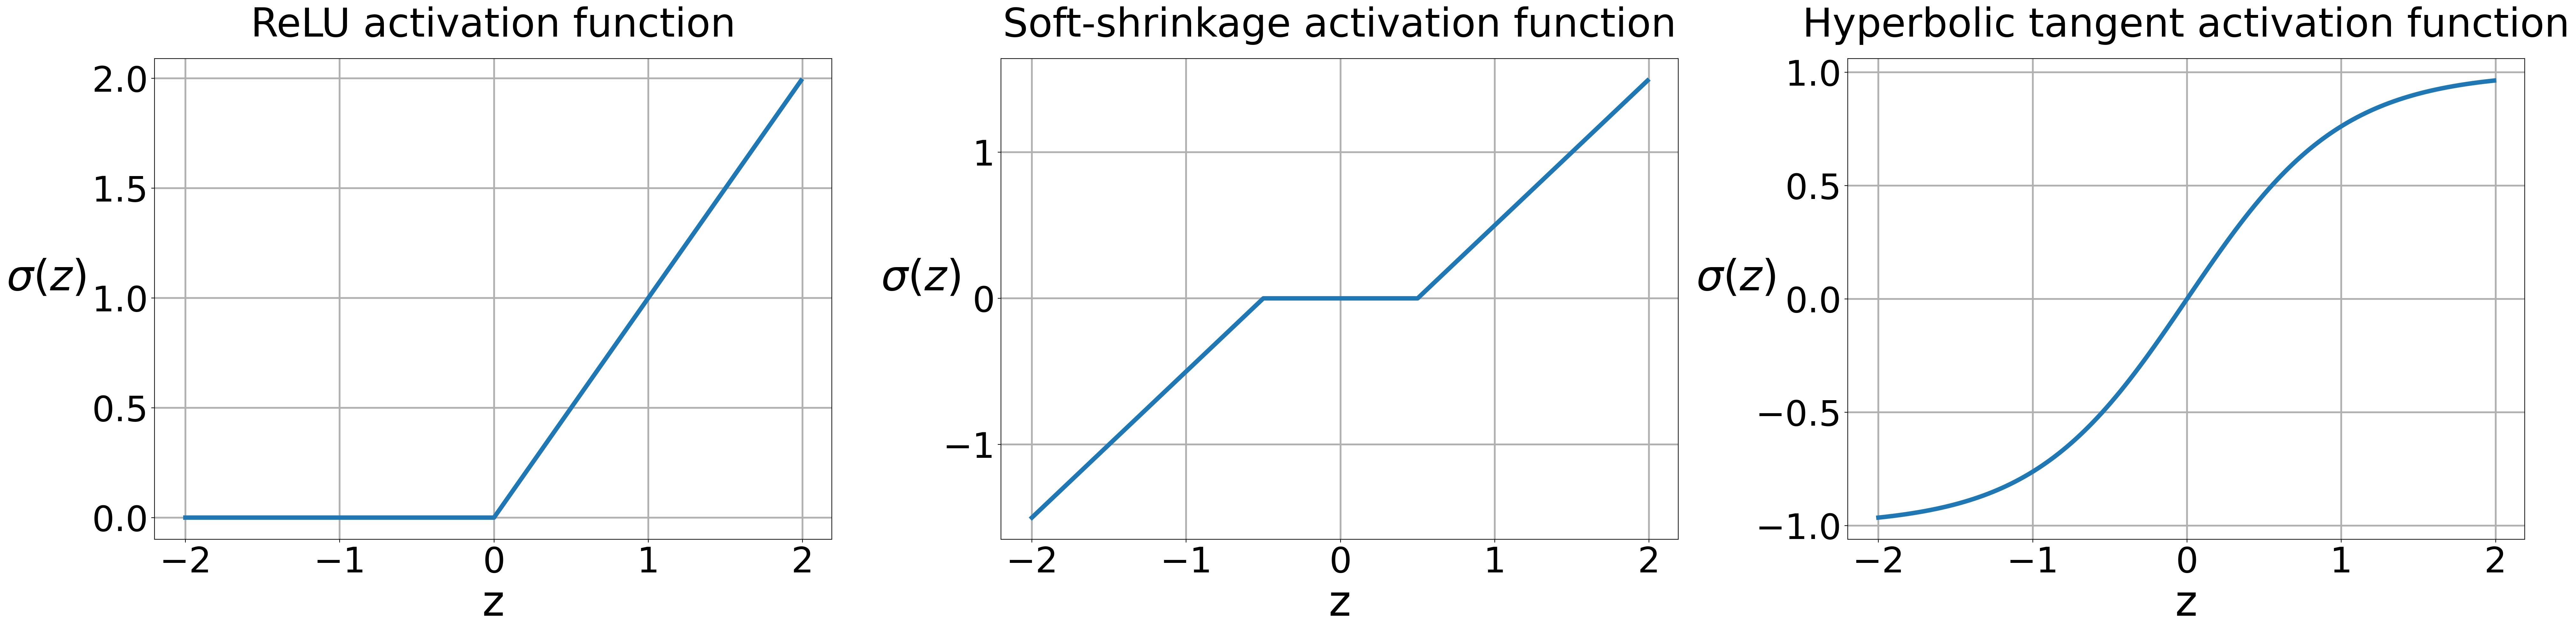
\includegraphics[width=0.9\textwidth]{lifted/all_three_activation_functions_bigger_font.png}
    
    \vspace{0.5em}
    \small ReLU, soft-thresholding, and hyperbolic tangent all fit the same proximal-activation perspective used by the lifted Bregman framework.
\end{frame}

\begin{frame}{Why the Bregman Loss is Different}
    \centering
    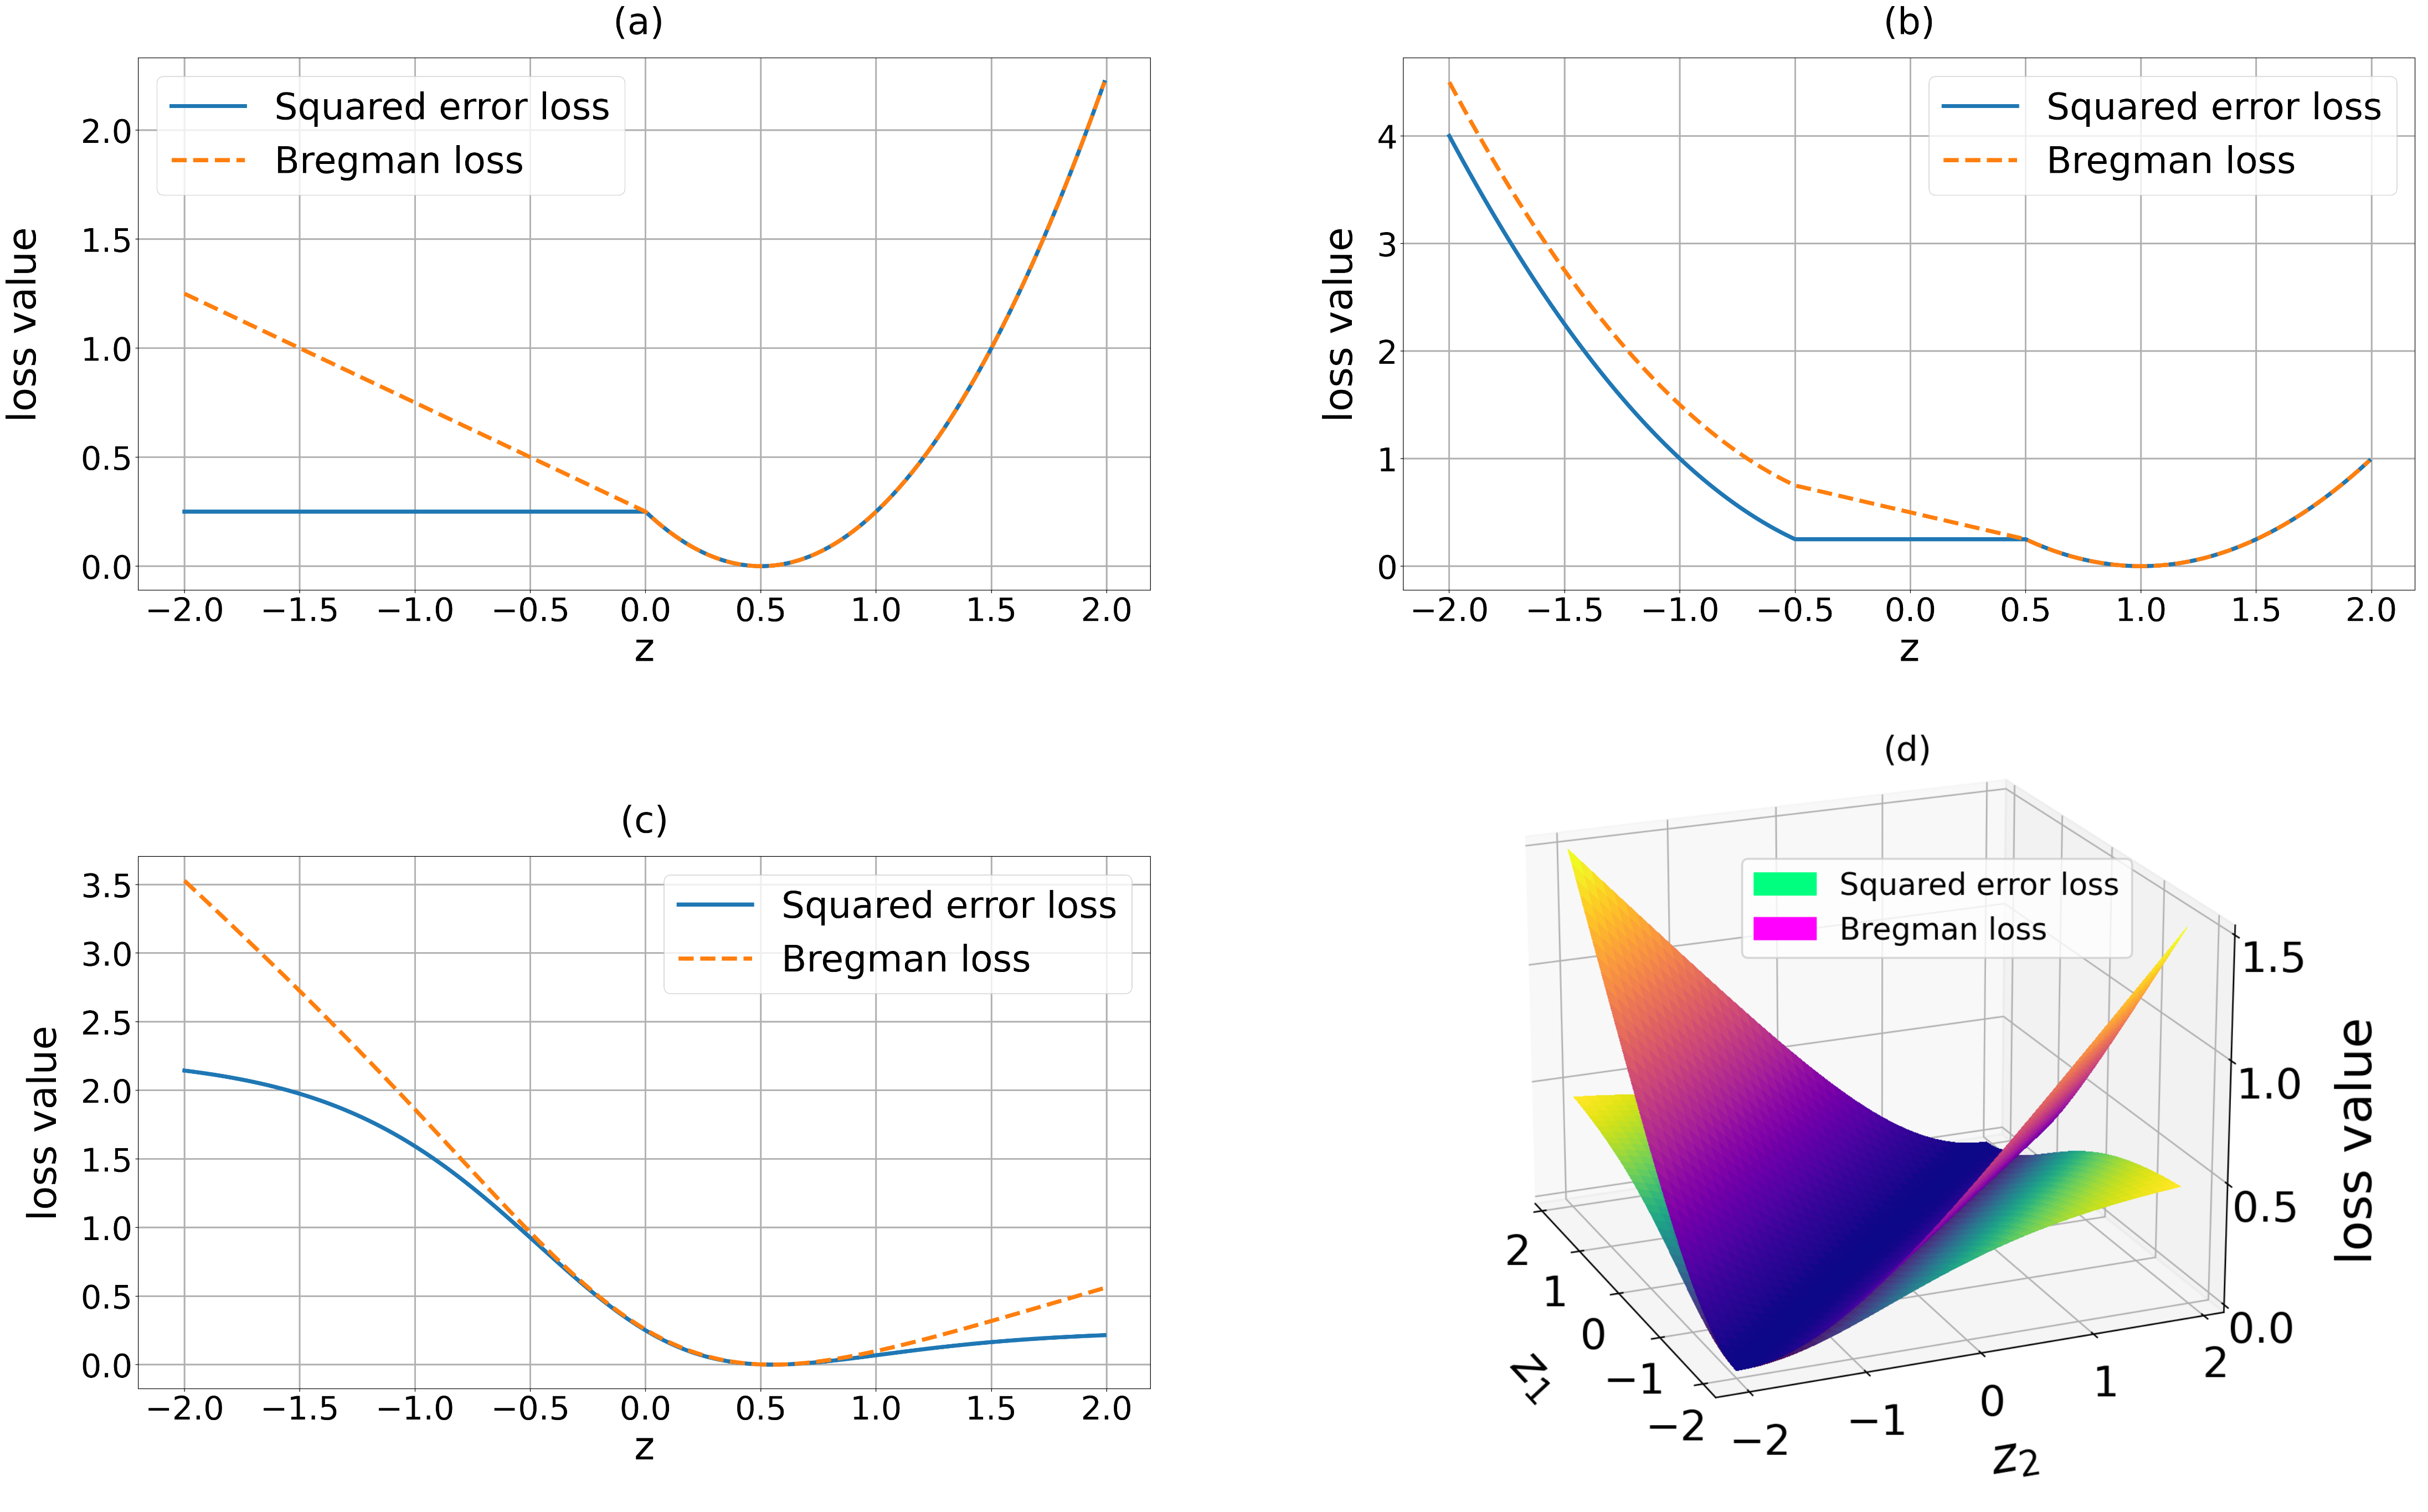
\includegraphics[width=0.55\textwidth]{lifted/Bregman_loss_plots_bigger_font.png}
    
    \vspace{0.5em}
    \small The Bregman penalties are not just quadratic surrogates: they adapt to the activation geometry and enforce the correct proximal consistency condition.
\end{frame}

% ==============================================================================
\section{Generalised Perceptron Learning}
% ==============================================================================

\begin{frame}{Generalised Perceptron Learning}
    To see this in action minimally, let's revisit Rosenblatt's classical perceptron through the lifted Bregman lens. 
    
    \vspace{1em}
    Consider a one-layer model:
    $$ \hat y = \sigma\left(W^\top x + b\right) $$
    where $\sigma = \operatorname{prox}_{\Psi}$. 
    
    \vspace{1em}
    We can decouple the nonlinearity through auxiliary variables and penalise consistency with a Bregman gap.
\end{frame}

\begin{frame}{Perceptron Bregman Objective}
    For training samples $\{(x^i,y^i)\}_{i=1}^s$, we consider the objective:
    
    \begin{theoremblock}{Regularised Perceptron Objective}
    $$ \min_{W,b}\; \frac{1}{s}\sum_{i=1}^s B_{\Psi}\!\left(y^i, W^\top x^i + b\right) + \alpha\,R(W,b) $$
    \end{theoremblock}
    
    Where $R(W,b)$ could be $\|W\|_1$ for sparsity, or $\frac12\|W\|_F^2$ for Tikhonov stabilisation.
    
    Because $\nabla_z B_{\Psi}(x, z) = \sigma(z) - x$, the gradients with respect to $W$ and $b$ follow from the affine map alone.
\end{frame}

\begin{frame}{Generalised Rosenblatt Update}
    When $R \equiv 0$, incremental or mini-batch gradient descent yields the \textbf{Generalised Rosenblatt Update}.
    
    \begin{algorithm}[H]
    \caption{Generalised Rosenblatt Update (Bregman Loss)}\label{alg:generalised_rosenblatt}
    \begin{algorithmic}
    \State \textbf{Input:} Initial $W^0, b^0$, step sizes $\{\tau_W^k\}, \{\tau_b^k\}$.
    \For{$k = 0,1,2,\ldots$}
        \State Choose mini-batch $B_k \subset \{1,\ldots,s\}$.
        \State $g_W^k = \frac{1}{|B_k|}\sum_{i\in B_k} x^i\left(\sigma\!\left((W^k)^\top x^i + b^k\right) - y^i\right)^\top$
        \State $g_b^k = \frac{1}{|B_k|}\sum_{i\in B_k} \left(\sigma\!\left((W^k)^\top x^i + b^k\right) - y^i\right)$
        \State $W^{k+1} = W^k - \tau_W^k g_W^k$
        \State $b^{k+1} = b^k - \tau_b^k g_b^k$
    \EndFor
    \end{algorithmic}
    \end{algorithm}
\end{frame}

\begin{frame}{Adding Sparsity: Rosenblatt-ISTA}
    If we include sparse regularisation $R(W,b)=\|W\|_1$, we obtain a direct Forward-Backward splitting scheme.
    
    \vspace{1em}
    The smooth part is the Bregman data term and the non-smooth part is the $\ell_1$ penalty, yielding an ISTA-type proximal step on the weights.

    \begin{block}{Interpretation}
        The update is now split into two conceptually clean stages:
        \begin{enumerate}
            \item a gradient step using the derivative-free Bregman signal,
            \item a proximal soft-thresholding step promoting sparsity.
        \end{enumerate}
    \end{block}
\end{frame}

\begin{frame}{Rosenblatt-ISTA Algorithm}
    \begin{algorithm}[H]
    \caption{Rosenblatt-ISTA for Sparse Perceptrons}\label{alg:rosenblatt_ista}
    \begin{algorithmic}
    \State \textbf{Input:} Initial $W^0, b^0$, step sizes $\{\tau_W^k\}, \{\tau_b^k\}$, regularisation $\alpha>0$.
    \For{$k = 0,1,2,\ldots$}
        \State $g_W^k = \frac{1}{|B_k|}\sum_{i\in B_k} x^i\left(\sigma\!\left((W^k)^\top x^i + b^k\right) - y^i\right)^\top$
        \State $g_b^k = \frac{1}{|B_k|}\sum_{i\in B_k} \left(\sigma\!\left((W^k)^\top x^i + b^k\right) - y^i\right)$
        \State $\widetilde W^{k+1} = W^k - \tau_W^k g_W^k$
        \State ${\color{uclred} W^{k+1} = \operatorname{prox}_{\tau_W^k\alpha\|\cdot\|_1}(\widetilde W^{k+1}) }$ \Comment{Soft-Thresholding}
        \State $b^{k+1} = b^k - \tau_b^k g_b^k$
    \EndFor
    \end{algorithmic}
    \end{algorithm}
\end{frame}

\begin{frame}{Numerical Snapshot: Sparse Perceptron Training}
    \begin{columns}[T,totalwidth=\textwidth]
        \column{0.49\textwidth}
        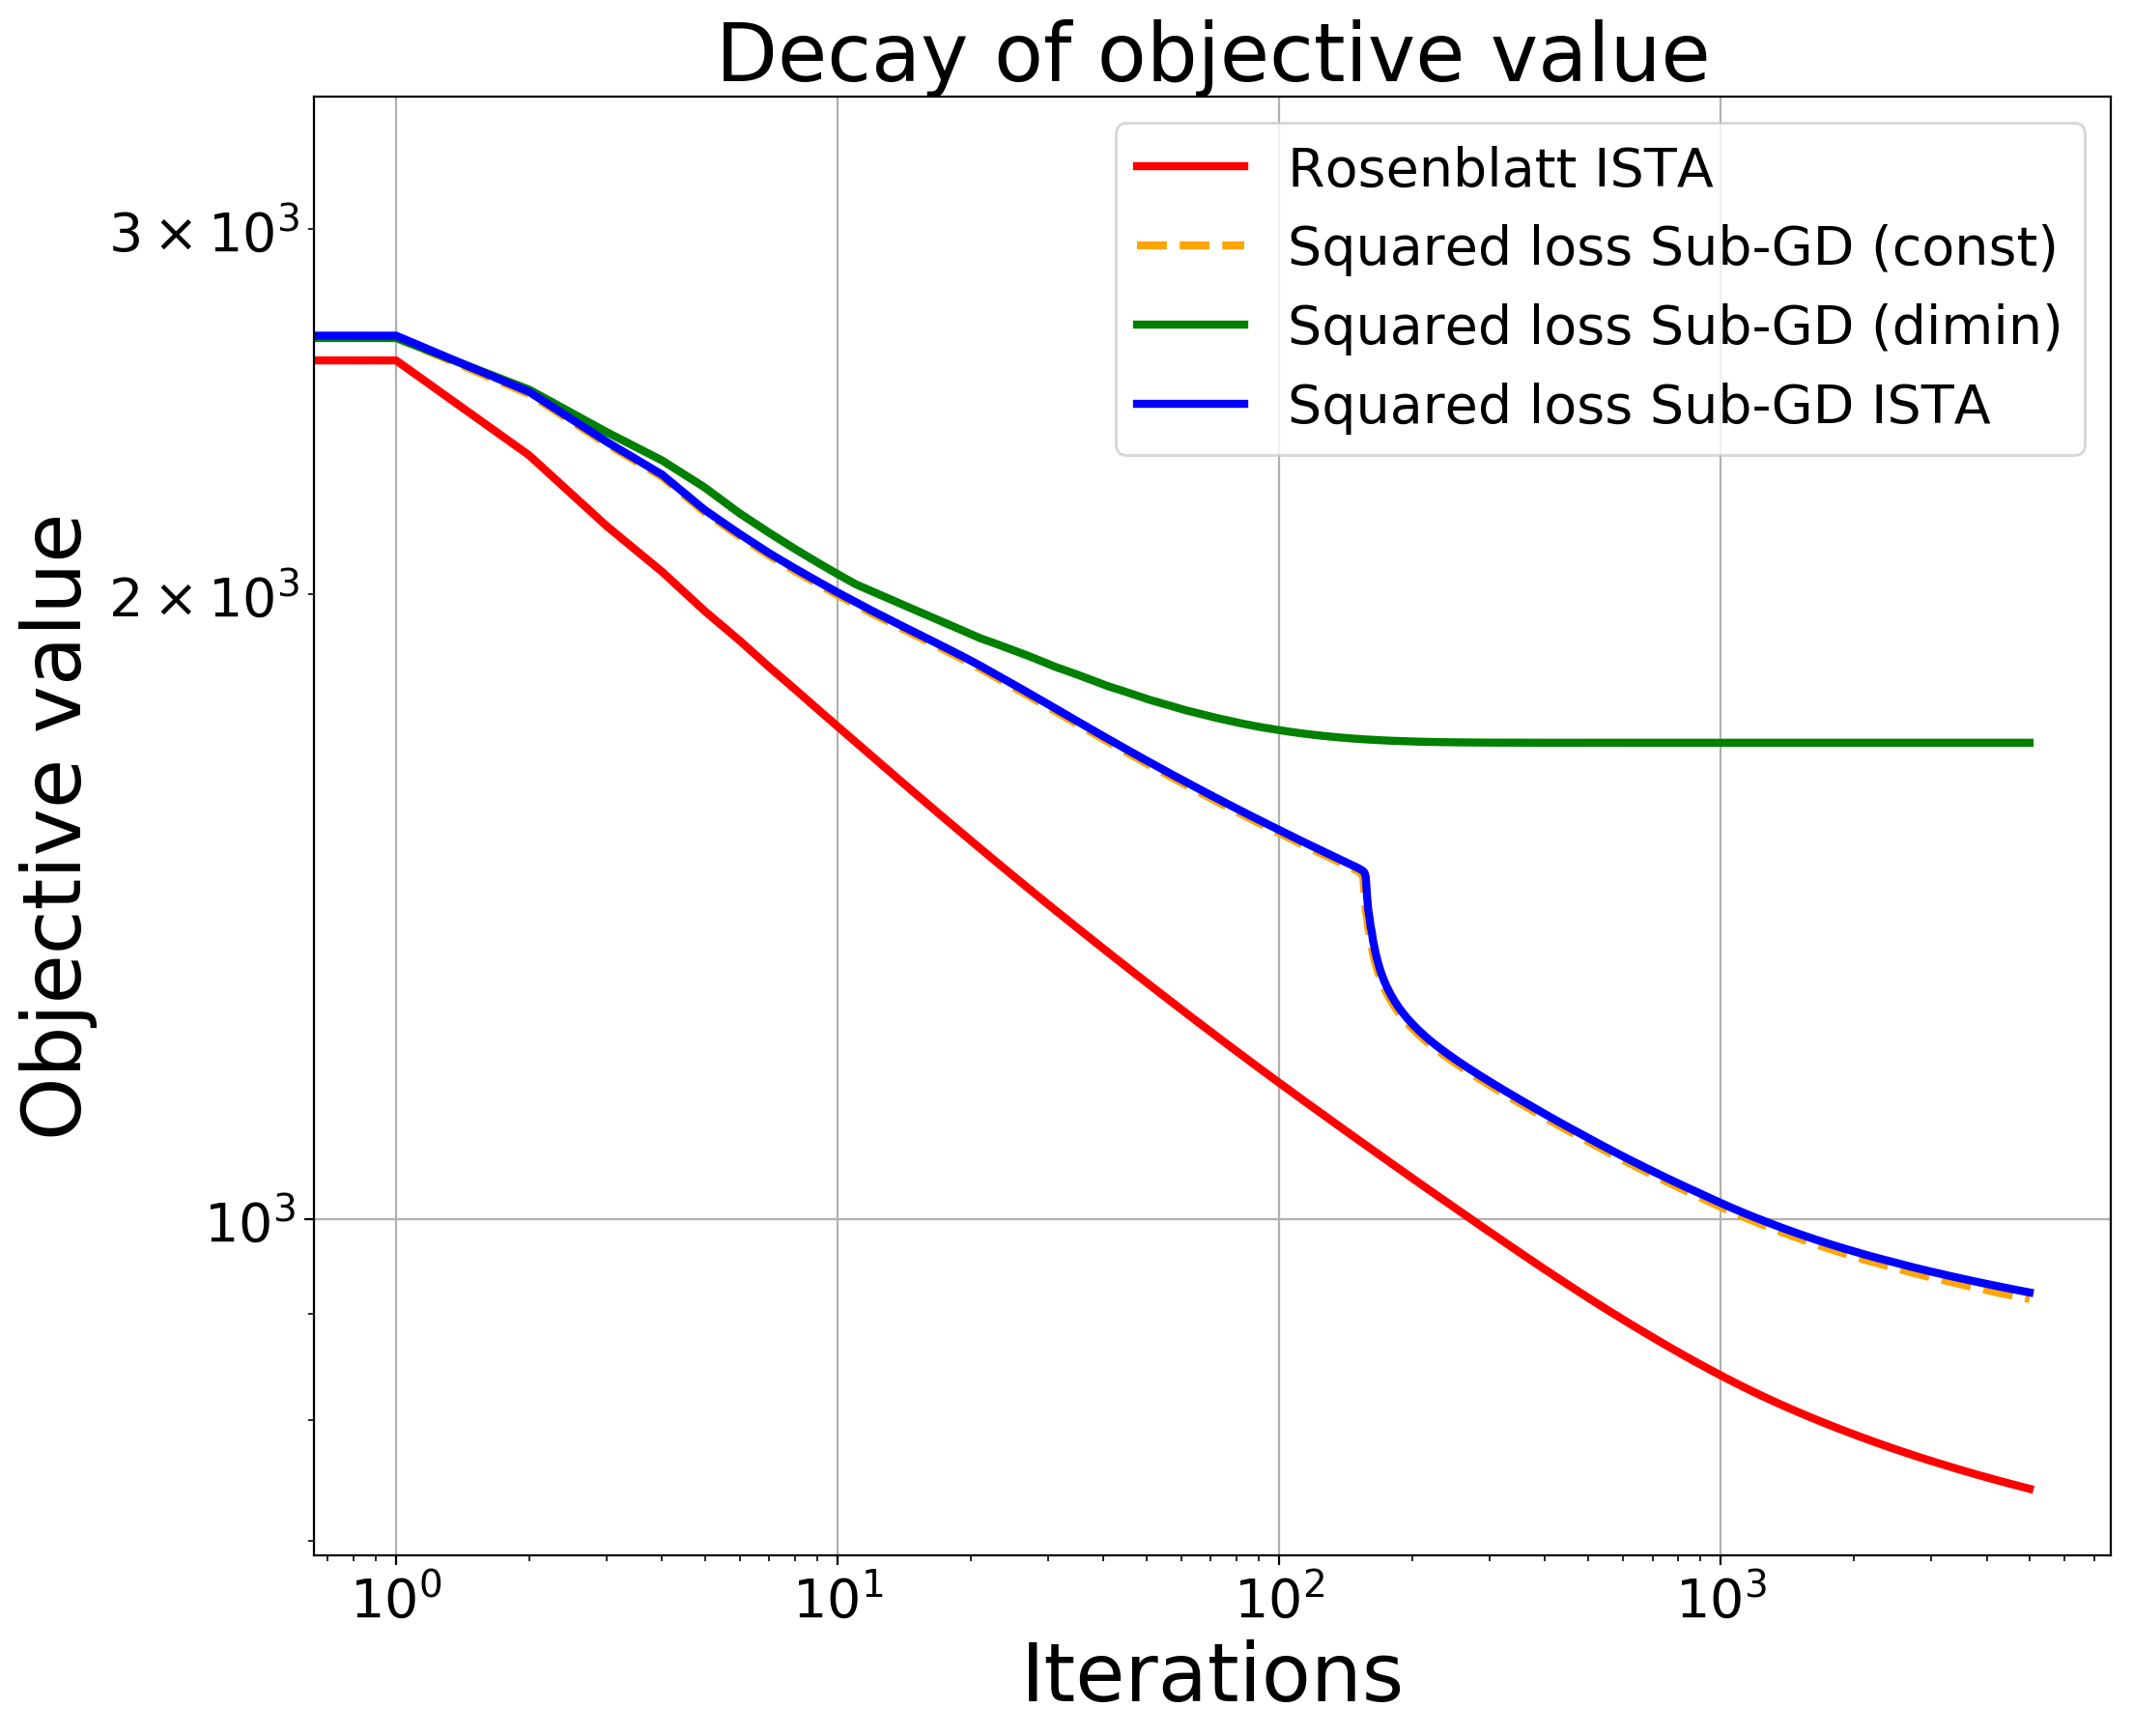
\includegraphics[width=\textwidth]{lifted/rosenblatt_ista_fmnist_obj_over_iterations_logx.png}

        \column{0.49\textwidth}
        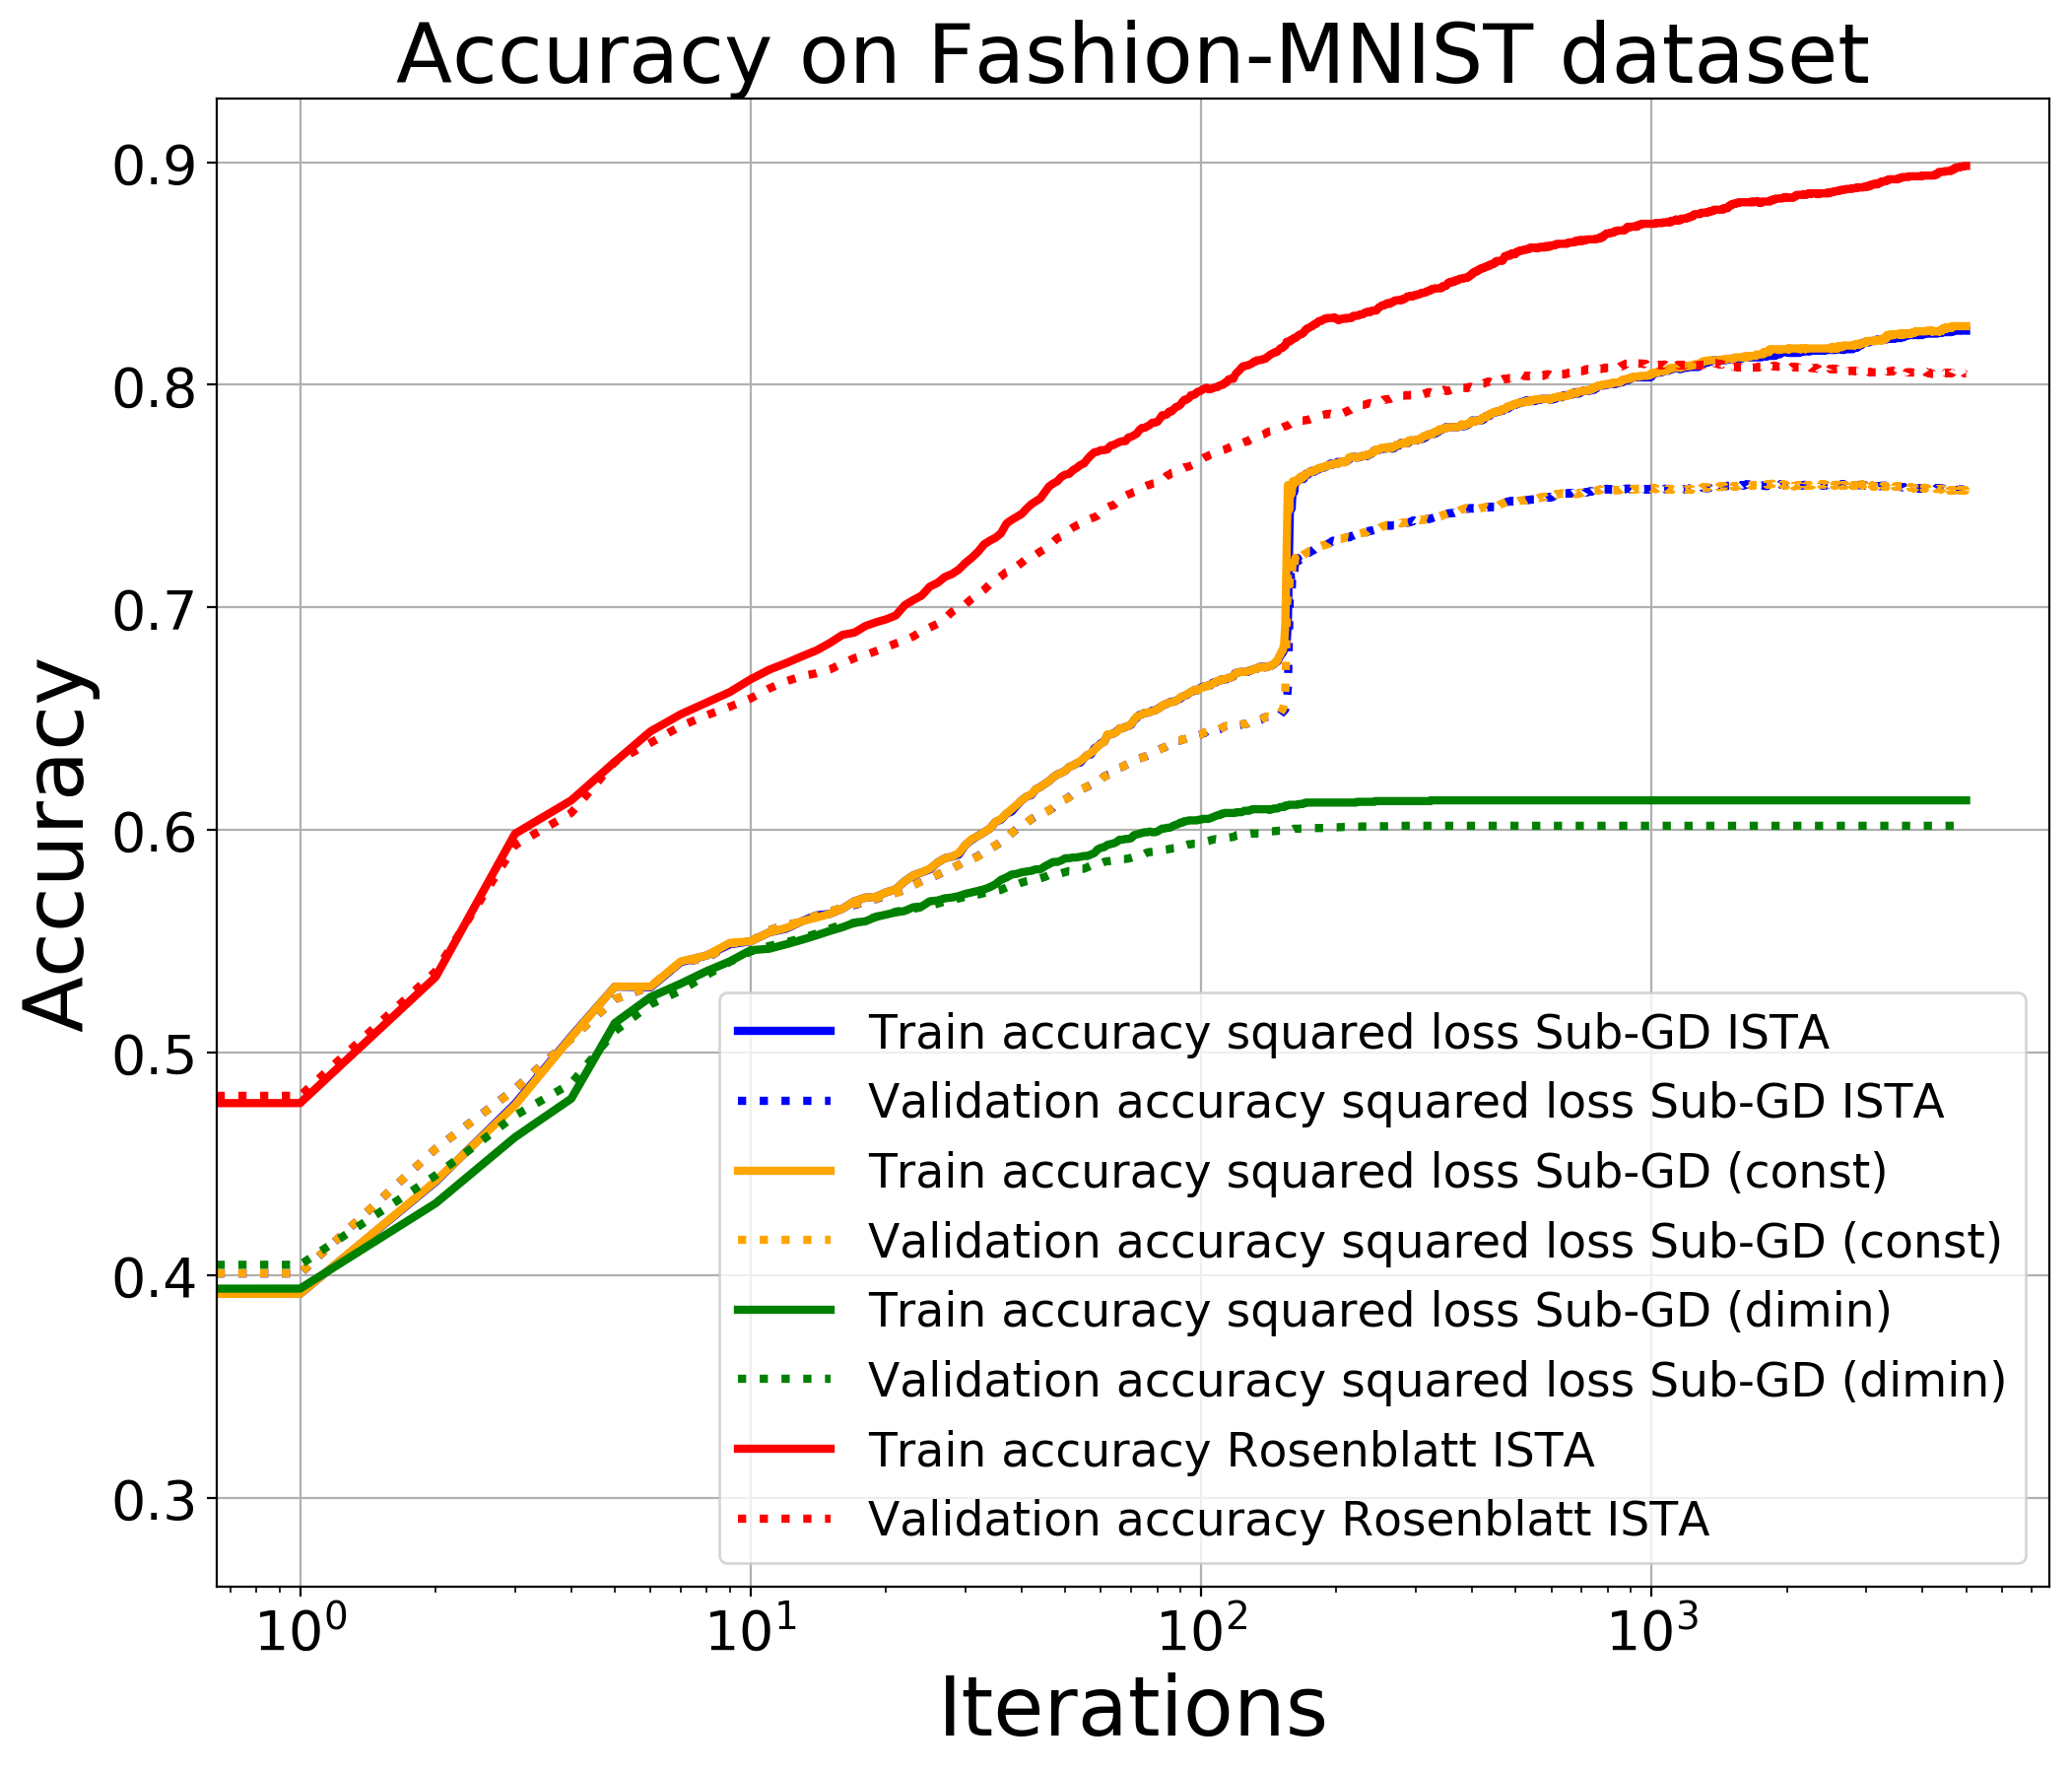
\includegraphics[width=\textwidth]{lifted/rosenblatt_ista_fmnist_acc_over_iterations_logx.png}
    \end{columns}

    \vspace{0.5em}
    \begin{block}{What to notice}
        These Fashion-MNIST experiments from \cite{wangbenning2020generalised} show both optimisation progress and predictive quality: the Bregman-based sparse perceptron update reduces the objective while maintaining competitive training and validation accuracy.
    \end{block}
\end{frame}

\begin{frame}{Summary: Lecture 1}
    \begin{itemize}
        \item \textbf{The Bottleneck:} Standard back-propagation restricts training due to sequential locking and necessitates sub-gradient heuristics for non-smooth functions.
        \item \textbf{Lifting the Problem:} By introducing auxiliary layer variables, we can formulate training as a parallelisable, block-coordinate descent problem.
        \item \textbf{The Bregman Solution:} Classical lifting suffers from affine degeneracy. The \textbf{Lifted Bregman Framework} uses Fenchel-Young gaps to strictly enforce proximal activations \textit{without} computing their derivatives.
        \item \textbf{Next Time:} We will generalise this framework into a unified block-operator architecture covering ResNets, MLPs, and Unrolled Networks!
    \end{itemize}
\end{frame}

\begin{frame}[allowframebreaks]{References}
    \bibliographystyle{abbrv}
    \bibliography{../../Lecture_Notes/references}
\end{frame}

\end{document}